\documentclass{standalone}
\usepackage{fkmath}
\usepackage{tikz, tikz-3dplot}
\usetikzlibrary{decorations.pathreplacing}
\begin{document}

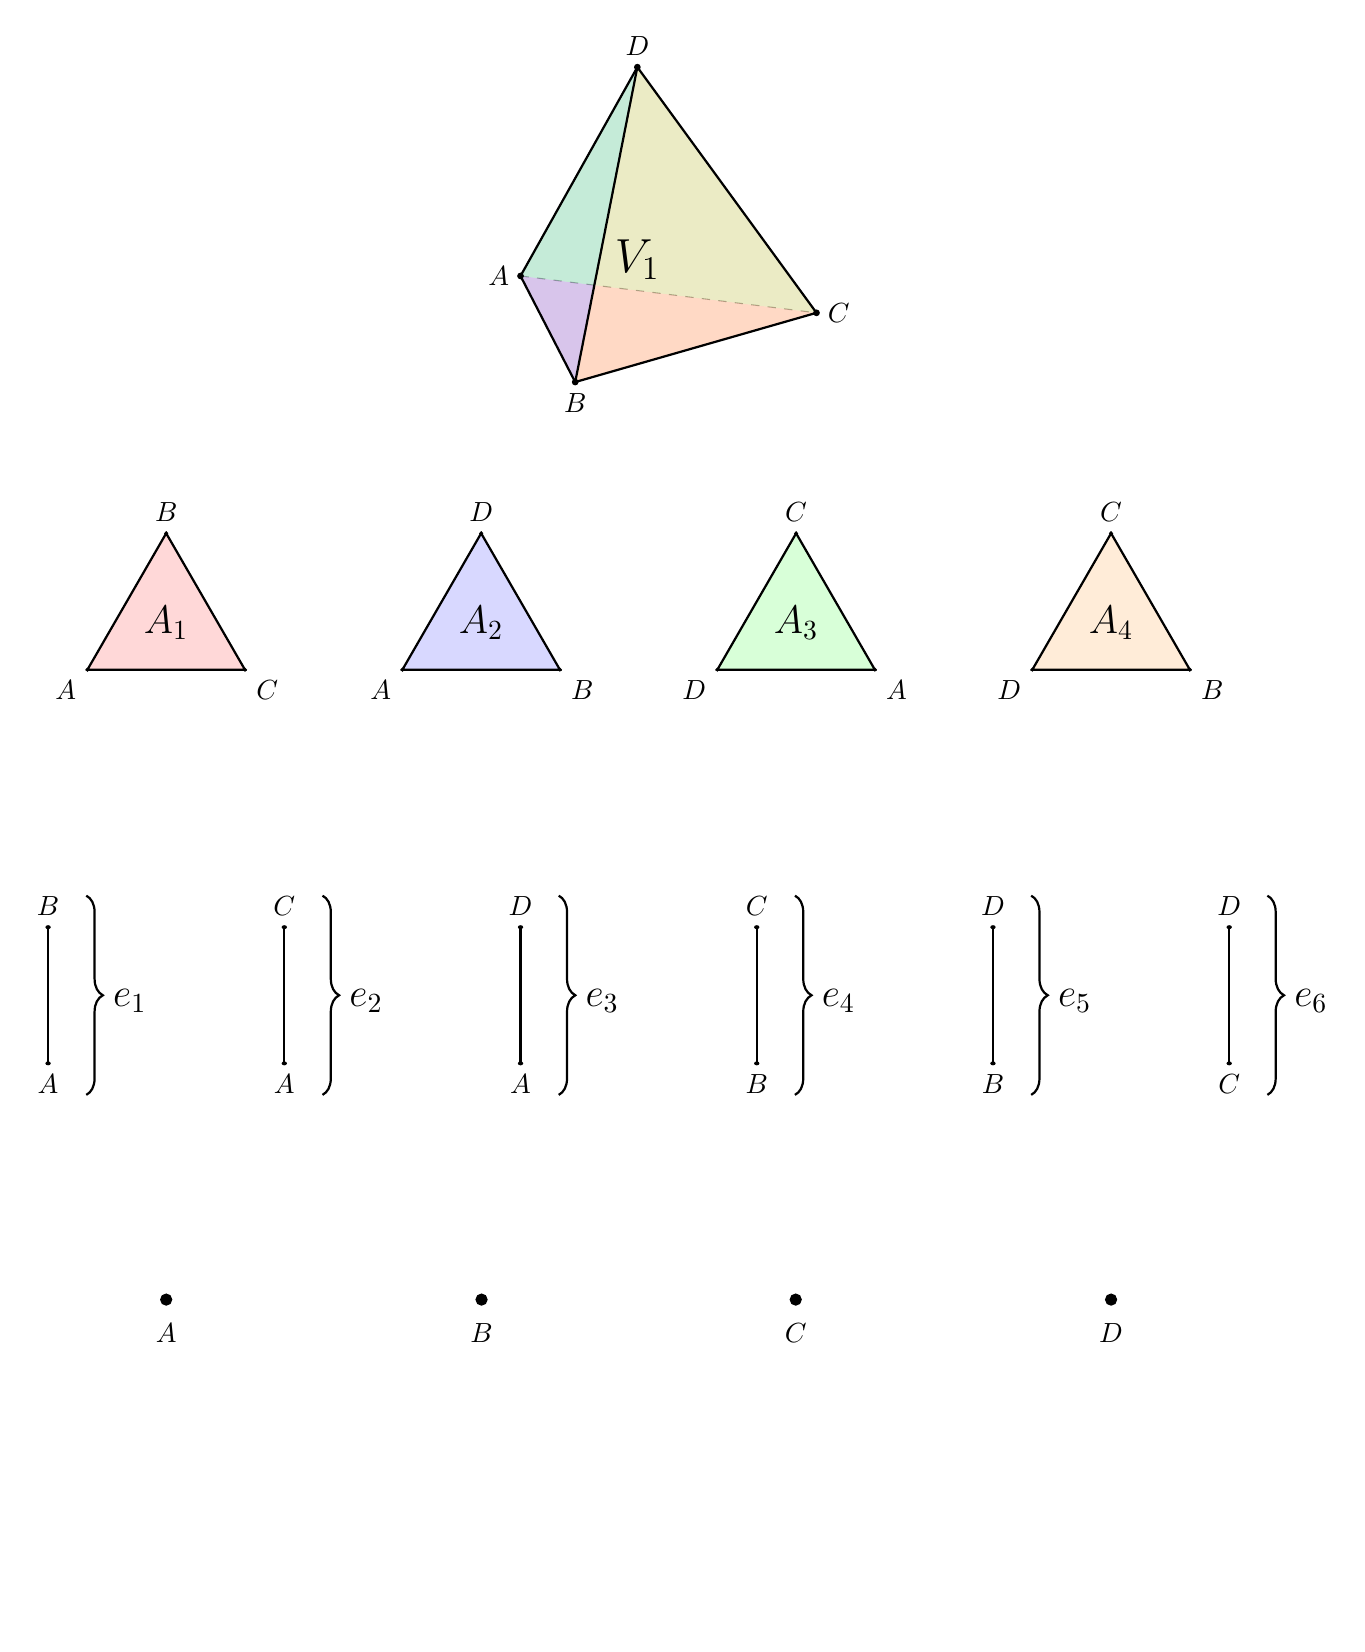
\begin{tikzpicture}

  % How far apart, in cm, to space the sub-figure portions
  \pgfmathsetmacro{\ysep}{4}


  \tdplotsetmaincoords{70}{80}
  \begin{scope}[tdplot_main_coords, scale=2, xshift=-.25cm, yshift=.5cm]
    \path
    coordinate (A) at (0,0,0)
    coordinate (B) at (2,0,0)
    coordinate (C) at (1,1.732,0)
    coordinate (D) at (1,.577,1.733);

    \draw [dashed] (A)--(C);
    \fill [opacity=.5, red!30!white] (A) -- (B) -- (C) -- cycle;
    \fill [opacity=.5, blue!30!white] (D) -- (B) -- (A) -- cycle;
    \fill [opacity=.5, green!30!white] (D) -- (A) -- (C) -- cycle;
    \draw[thick] (A) -- (B) (A) -- (D);
    \draw[thick, fill opacity=.5, fill=orange!30!white] (D) -- (B) -- (C) -- cycle;

    \node (V) at (1,.577,.433) {\LARGE $V_1$};

    \foreach \v/\position in {A/left,B/below,C/right,D/above} {
      \draw[fill=black] (\v) circle (0.5pt) node [\position=0.2mm] {$\v$};
    }
  \end{scope}

  % Shift all the 2-simplices down by 4 cm
  \begin{scope}[yshift=-\ysep cm]
    \begin{scope}[xshift=-6cm]

      \path
      coordinate (A) at (0,0)
      coordinate (C) at (2,0)
      coordinate (B) at (1,1.732);

      \draw[thick, fill opacity=.5, fill=red!30!white] (A) -- (B) -- (C) -- cycle;

      \node (A1) at (1,.6) {\Large $A_1$};

      \foreach \v/\position in {A/below left, C/below right, B/above} {
        \draw[fill=black] (\v) circle (0.5pt) node [\position=0.2mm] {$\v$};
      }
    \end{scope}

    \begin{scope}[xshift=-2cm]
      \path
      coordinate (A) at (0,0)
      coordinate (B) at (2,0)
      coordinate (D) at (1,1.732);

      \draw[thick, fill opacity=.5, fill=blue!30!white] (D) -- (B) -- (A) -- cycle;

      \node (A2) at (1,.6) {\Large $A_2$};

      \foreach \v/\position in {A/below left, B/below right, D/above} {
        \draw[fill=black] (\v) circle (0.5pt) node [\position=0.2mm] {$\v$};
      }
    \end{scope}

    \begin{scope}[xshift=2cm]
      \path
      coordinate (D) at (0,0)
      coordinate (A) at (2,0)
      coordinate (C) at (1,1.732);

      \draw[thick, fill opacity=.5, fill=green!30!white] (D) -- (A) -- (C) -- cycle;

      \node (A3) at (1,.6) {\Large $A_3$};

      \foreach \v/\position in {D/below left, A/below right, C/above} {
        \draw[fill=black] (\v) circle (0.5pt) node [\position=0.2mm] {$\v$};
      }
    \end{scope}

    \begin{scope}[xshift=6cm]
      \path
      coordinate (D) at (0,0)
      coordinate (B) at (2,0)
      coordinate (C) at (1,1.732);

      \draw[thick, fill opacity=.5, fill=orange!30!white] (D) -- (B) -- (C) -- cycle;

      \node (A4) at (1,.6) {\Large $A_4$};

      \foreach \v/\position in {D/below left, B/below right, C/above} {
        \draw[fill=black] (\v) circle (0.5pt) node [\position=0.2mm] {$\v$};
      }
    \end{scope}
  \end{scope}

  % The 1-simplices
  \begin{scope}[yshift=-2.25 * \ysep cm, xshift=1cm, xscale=1.5]
    \tikzset{
      brace/.style={
        thick,
        decoration={brace, mirror, raise=1pt, amplitude=6pt},
        decorate
      },
      blabel/.style={
        right, pos=.5, xshift=7pt, yshift=-2pt
      }
    }
    \begin{scope}[xshift=-5cm]
      \def\firstcoord{A}
      \def\secondcoord{B}
      \path coordinate (\firstcoord) at (0,0) coordinate (\secondcoord) at (0,1.73);
      \draw[thick] (\firstcoord) -- (\secondcoord);

      \draw[brace] (.3,-.4) -- node[blabel] {\Large $e_1$} (.3,2.13);

      \foreach \v/\position in {\firstcoord/below, \secondcoord/above} {
        \draw[fill=black] (\v) circle (0.5pt) node [\position=0.2mm] {$\v$};
      }
    \end{scope}

    \begin{scope}[xshift=-3cm]
      \def\firstcoord{A}
      \def\secondcoord{C}
      \path coordinate (\firstcoord) at (0,0) coordinate (\secondcoord) at (0,1.73);
      \draw[thick] (\firstcoord) -- (\secondcoord);

      \draw[brace] (.3,-.4) -- node[blabel] {\Large $e_2$} (.3,2.13);

      \foreach \v/\position in {\firstcoord/below, \secondcoord/above} {
        \draw[fill=black] (\v) circle (0.5pt) node [\position=0.2mm] {$\v$};
      }
    \end{scope}

    \begin{scope}[xshift=-1cm]
      \def\firstcoord{A}
      \def\secondcoord{D}
      \path coordinate (\firstcoord) at (0,0) coordinate (\secondcoord) at (0,1.73);
      \draw[thick] (\firstcoord) -- (\secondcoord);

      \draw[brace] (.3,-.4) -- node[blabel] {\Large $e_3$} (.3,2.13);

      \foreach \v/\position in {\firstcoord/below, \secondcoord/above} {
        \draw[fill=black] (\v) circle (0.5pt) node [\position=0.2mm] {$\v$};
      }
    \end{scope}

    \begin{scope}[xshift=1cm]
      \def\firstcoord{B}
      \def\secondcoord{C}
      \path coordinate (\firstcoord) at (0,0) coordinate (\secondcoord) at (0,1.73);
      \draw[thick] (\firstcoord) -- (\secondcoord);

      \draw[brace] (.3,-.4) -- node[blabel] {\Large $e_4$} (.3,2.13);

      \foreach \v/\position in {\firstcoord/below, \secondcoord/above} {
        \draw[fill=black] (\v) circle (0.5pt) node [\position=0.2mm] {$\v$};
      }
    \end{scope}

    \begin{scope}[xshift=3cm]
      \def\firstcoord{B}
      \def\secondcoord{D}
      \path coordinate (\firstcoord) at (0,0) coordinate (\secondcoord) at (0,1.73);
      \draw[thick] (\firstcoord) -- (\secondcoord);

      \draw[brace] (.3,-.4) -- node[blabel] {\Large $e_5$} (.3,2.13);

      \foreach \v/\position in {\firstcoord/below, \secondcoord/above} {
        \draw[fill=black] (\v) circle (0.5pt) node [\position=0.2mm] {$\v$};
      }
    \end{scope}

    \begin{scope}[xshift=5cm]
      \def\firstcoord{C}
      \def\secondcoord{D}
      \path coordinate (\firstcoord) at (0,0) coordinate (\secondcoord) at (0,1.73);
      \draw[thick] (\firstcoord) -- (\secondcoord);

      \draw[brace] (.3,-.4) -- node[blabel] {\Large $e_6$} (.3,2.13);

      \foreach \v/\position in {\firstcoord/below, \secondcoord/above} {
        \draw[fill=black] (\v) circle (0.5pt) node [\position=0.2mm] {$\v$};
      }
    \end{scope}
  \end{scope}

  \begin{scope}[yshift=-3 * \ysep cm, xshift=1cm, x=1.5cm]
    \path
    coordinate (A) at (-4,0)
    coordinate (B) at (-1.33,0)
    coordinate (C) at (1.33,0)
    coordinate (D) at (4,0);

    \foreach \v in {A,B,C,D} {
      \draw[fill=black] (\v) circle (2pt) node [below, yshift=-5pt] {$\v$};
    }
  \end{scope}

  % Empty set
  \node () at (1, -4*\ysep) {\LARGE $\set{}$};

\end{tikzpicture}

\end{document}
